%\documentclass[10pt,a4paper]{article}
\documentclass[10pt,a4paper]{scrreprt}
\usepackage[utf8]{inputenc}
\usepackage{amsmath}
\usepackage{amsfonts}
\usepackage{amssymb}
\usepackage{graphicx}
\usepackage[left=2cm,right=2cm,top=2cm,bottom=2cm]{geometry}

\usepackage{bm}

\usepackage{pythonhighlight}

% integral d
\newcommand{\myd}{\;\mathrm{d}}
% overbar
\newcommand{\overbar}[1]{\mkern 1.5mu\overline{\mkern-1.5mu#1\mkern-1.5mu}\mkern 1.5mu}

\author{Yi Hu}
\title{Homogenization for Multi Field Modelling}
\subtitle{Part II: Implementation and Numerical Examples}

\begin{document}
\chapter{Numerical Examples}
In this part some numerical examples using this module is presented. First different kinds of inclusions are listed. Then 2d and 3d examples both in uni field and multi field modelling are given. At the end of this part the usage of the module is given in the IPython environment.

\section{Various Inclusions}
\begin{figure}[h]
\centering
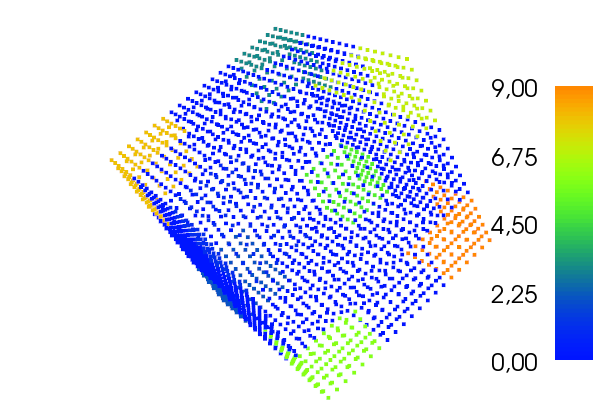
\includegraphics[scale=0.4]{/home/yihu/studien_arbeit_fenics/report/pics/dolfin_plot_2.png}
\caption{Typical free energy profile}
\label{fig:meta}
\end{figure}

[fig: inclusion and geometry 2d, 3d, different inclusions]

\section{2D Modelling}
[fig: 2d uni fluctuation, strain, stress]

[fig: 2d multi]

\section{3D Modelling}
[fig: 3d uni]

[fig: 3d multi]

\section{Simulation Template}
\begin{python}
from dolfin import *

import numpy as np

import cell_geom as geom
import cell_material as mat
import cell_computation as comp

parameters['linear_algebra_backend'] = 'Eigen'

mesh = Mesh(r'./m_fine.xml')

cell = geom.UnitCell(mesh)

inc = geom.InclusionCircle(2, (0.5, 0.5), 0.25)
inc_di = {'circle_inc': inc}
cell.set_append_inclusion(inc_di)

E_m, nu_m, E_i, nu_i = 10.0, 0.3, 1000.0, 0.3
mat_m = mat.st_venant_kirchhoff(E_m, nu_m)
mat_i = mat.st_venant_kirchhoff(E_i, nu_i)
mat_li = [mat_m, mat_i]
VFS = VectorFunctionSpace(cell.mesh, "CG", 1, 
                          constrained_domain=geom.PeriodicBoundary_no_corner(2))

def deform_grad_with_macro(F_bar, w_component):
    return F_bar + grad(w_component)

w = Function(VFS)
strain_space = TensorFunctionSpace(mesh, 'DG', 0)
compute = comp.MicroComputation(cell, mat_li, 
                                [deform_grad_with_macro],
                                [strain_space])

F_bar = [0.9, 0., 0., 1.]

compute.input([F_bar], [w])

comp.set_solver_parameters('non_lin_newton', lin_method='direct',
                      linear_solver='cholesky')


compute.comp_fluctuation(print_progress=True, print_solver_info=False)

compute.view_fluctuation()

delta = 0.01

for i in range(10):
    F_bar[0] -= delta
    print F_bar
    compute.input([F_bar], [w])
    compute.comp_fluctuation(print_progress=True, print_solver_info=False)
\end{python}

\section{Convergence Comparison with Finite Difference Calculation}

\section{Calculation till Instability}

\end{document}